\documentclass[tikz]{standalone}
\usepackage{tikz}
\usetikzlibrary{positioning}
\usetikzlibrary{calc}

\begin{document}

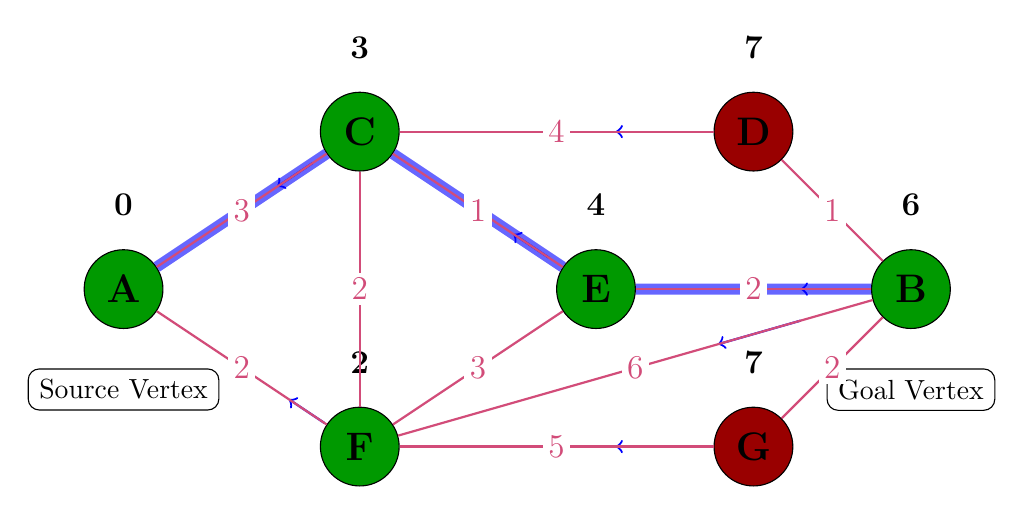
\begin{tikzpicture}[
    node distance=3cm,
    vertex/.style={circle, draw, fill=gray!70, minimum size=1cm, font=\Large\bfseries},
    edge/.style={draw, thick, color=purple!70},
    weight/.style={fill=white, inner sep=2pt, font=\large}
]

% Define node positions
\node[vertex, fill=green!60!black] (A) at (-4, 0) {A};
\node[vertex, fill=green!60!black] (C) at (-1, 2) {C};
\node[vertex, fill=green!60!black] (F) at (-1, -2) {F};
\node[vertex, fill=green!60!black] (E) at (2, 0) {E};
\node[vertex, fill=red!60!black] (D) at (4, 2) {D};
\node[vertex, fill=green!60!black] (B) at (6, 0) {B};
\node[vertex, fill=red!60!black] (G) at (4, -2) {G};

% Blue arrows for Picture 8 (pointing from child to parent)
\draw[->, blue, thick] ($ (D)!0.2!(C) $) -- ($ (D)!0.35!(C) $);
\draw[->, blue, thick] ($ (G)!0.2!(F) $) -- ($ (G)!0.35!(F) $);
\draw[->, blue, thick] ($ (C)!0.2!(A) $) -- ($ (C)!0.35!(A) $);
\draw[->, blue, thick] ($ (E)!0.2!(C) $) -- ($ (E)!0.35!(C) $);
\draw[->, blue, thick] ($ (B)!0.2!(E) $) -- ($ (B)!0.35!(E) $);
\draw[->, blue, thick] ($ (F)!0.15!(A) $) -- ($ (F)!0.3!(A) $);
\draw[->, blue, thick] ($ (B)!0.2!(F) $) -- ($ (B)!0.35!(F) $);

% Shortest path from B to A (thick partially transparent blue line)
\draw[blue, line width=4pt, opacity=0.6] (B) -- (E) -- (C) -- (A);

% Add distance labels above vertices
\node[above=0.3cm of A, font=\large\bfseries] {0};
\node[above=0.3cm of C, font=\large\bfseries] {3};
\node[above=0.3cm of F, font=\large\bfseries] {2};
\node[above=0.3cm of E, font=\large\bfseries] {4};
\node[above=0.3cm of D, font=\large\bfseries] {7};
\node[above=0.3cm of B, font=\large\bfseries] {6};
\node[above=0.3cm of G, font=\large\bfseries] {7};

% Add source vertex label
\node[below=0.5cm of A, draw, fill=white, rounded corners, inner sep=4pt] {Source Vertex};

% Add goal vertex label
\node[below=0.5cm of B, draw, fill=white, rounded corners, inner sep=4pt] {Goal Vertex};

% Draw edges with weights
\draw[edge] (A) -- (C) node[weight, midway] {3};
\draw[edge] (A) -- (F) node[weight, midway] {2};
\draw[edge] (C) -- (D) node[weight, midway] {4};
\draw[edge] (C) -- (E) node[weight, midway] {1};
\draw[edge] (C) -- (F) node[weight, midway] {2};
\draw[edge] (E) -- (F) node[weight, midway] {3};
\draw[edge] (E) -- (B) node[weight, midway] {2};
\draw[edge] (F) -- (B) node[weight, midway] {6};
\draw[edge] (D) -- (B) node[weight, midway] {1};
\draw[edge] (B) -- (G) node[weight, midway] {2};
\draw[edge] (F) -- (G) node[weight, midway] {5};

\end{tikzpicture}

\end{document} 